\chapter{Simulation Software Manual \& Technical Details}

The repository of the software code is available online at: \url{https://gitlab.com/doronbehar/lab-ion-trap-simulations}

The repository consists of several Python executable scripts, each with a different role. The main important scripts are \texttt{sim.py} and \texttt{plot.py}. Running \texttt{./sim.py} creates a set of \texttt{.h5} suffixed files (in HDF5\cite{HDF5} format), and running \texttt{./plot.py} with the \texttt{.h5} files as arguments opens an interactive window as depicted in figure~\ref{fig:software-plot-example}.

Most other scripts in the repository implement functionalities required for simulating, and can also be executed as standalone scripts as well. Executing them tests the functionality they implement, sometimes via printing numbers, and sometimes via opening complex interactive plots like in figures \ref{fig:mathieu-mass-dep} \& \ref{fig:pure-mathieu-coefficients}. The following sections will simply describe each script, hopefully in an order that will make it easy to understand the complete architecture of the repository.

\section{\texttt{flake.nix}: Setting up a Development Environment}

Before we'll begin describing the actual Python scripts, it is important to setup a proper development environment for running the scripts. The best software I'd recommend for any task for managing a development environment on a per-project basis, is the package manager \textit{Nix}\cite{Nix}. Nix is a functional package manager\cite{NixThesis}, meaning it is capable of producing (packages and) development environments from a pure set of inputs. The intention is to increase the likelihood that the resulted development environment will be reproducible\cite{SoftwareReproducitilityThesis} on any computer running Nix.

The main file that defines the development environment is \texttt{flake.nix}. If you have \texttt{nix} installed you should be able to run \texttt{nix develop}\footnote{Don't forget to enable the (currently, as of writing) \texttt{experimental-features = nix-command flakes}. See the relevant \href{https://nix.dev/manual/nix/stable/contributing/experimental-features}{Nix' Manual page} for more details.} in a command line shell and enter a Bash shell that would be capable of running any script in the repository just like I did - with the same versions of Python dependencies, and same LAMMPS version and build variant.

Don't decry these development environment instructions. Many crucial details and features in the Python scripts depend on specially built variants of the Python dependencies. Worth noting, are:

\begin{itemize}
	\item 2 important Matplotlib patches. Without 1 of the patches, \texttt{./plot.py} won't work at all.
	\item An unreleased version of a Python dependency called \texttt{pint}, including another patch for it not accepted upstream.
	\item The \texttt{lammps} package built with very specific CMake flags that make the simulations run faster.
	\item A TeXLive distribution with specific dependencies that are necessary to create all the LaTeX generated texts in the plots.
\end{itemize}

Nix can be installed on Darwin, and any GNU/Linux distribution, including \href{https://learn.microsoft.com/en-us/windows/wsl/install}{Windows' Subsystem for Linux} (WSL). I personally used \href{https://github.com/nix-community/NixOS-WSL}{NixOS on (WSL)} on the office's computer, with \href{https://gitlab.com/doronbehar/nixos-configs/-/blob/b540a8fef332ff64d0ae52a67ef96758b7d2b396/flake.nix#L104-134}{this} OS configuration, which also includes a few NVIDIA hardware settings which might be relevant if you want to actually enjoy GPU support by LAMMPS. The fact the operating system's settings are declared and are reproducible just as the development environment, is another outstanding feature of Nix.

To reduce the hassle of running \texttt{nix develop} every time you enter the repository's directory, I recommend using \href{https://direnv.net/}{\texttt{direnv}}, which is also supported on the same platforms as Nix. The following sections assume you have a working development environment set up.

\section{\texttt{sim.py}}

\texttt{sim.py} is the script that actually calls LAMMPS' shared object\footnote{Also referred to as \texttt{DLL} in MS windows terminology.}, and runs the simulation, while also saving the results into a set of \texttt{.h5} files. The full set of available command line options is printed when you run \texttt{./sim.py --help}, and is explained in general in this section.

\subsection{Parameters}

The total amount of simulation parameters is approximately 22. Most of them are of type float, some are booleans, and some are integers. Although some of the parameters are constants for most simulations, simply iterating the multi-dimensional space of the rest of the parameters is incomprehensible computationally. The sensible thing to do instead is to study the effects of a few parameters one by one, while other parameters are constant.

\texttt{./sim.py} is basically built with a command line option per parameter, enabling you to choose which parameters to scan. When a simulation parameter's command line option is not specified, either a specific, default single value is used, or a large set of parameter values are scanned. Hence, practically speaking you are forced to choose specific single values of some parameters, and the parameters neglected from the command, or given multiple values are the parameters scanned over, such that the scans are of 2-3 dimensions most of the time.

\subsubsection{Scanning-Enabled Parameters}\label{sssec:manual/multi-value-params}

Most of the float typed parameters' possible values are defined in \texttt{PARAMETERS\_INFO} defined in \texttt{physical\_constants.py}, along with complementary metadata per parameter. For example the set of initial temperatures is marked as \texttt{T\_init}, and possible values are $[5,10,20,40,80]\mathrm{K}$, defined using \texttt{numpy.geomspace}. Similar ranges are defined for other parameters.

When you run \texttt{./sim.py} and you want to choose specific values of a certain float like parameter, you use the indices of the array's values defined in \texttt{PARAMETERS\_INFO}. For example to scan the initial temperatures $[10,40]\mathrm{K}$, you would use \texttt{--T\_init 1 3}. If you want to specify a certain range of values, you can use Bash shell syntax to choose e.g $[5,10,20]\mathrm{K}$ with \texttt{--T\_init \{0..2\}}, which simply is expanded by Bash to \texttt{--T\_init 0 1 2}.

To view all available parameters and their values, \texttt{./sim.py --list} can be used, which lists all available parameters to the terminal in 2 tables. Tables \ref{tbl:sim-list-most} and \ref{tbl:sim-list-amounts} serve as a LaTeX copy of these tables. Eventually, to run scans with a sensible amount of varying parameters (2-3 dimensions), you'd need to write \texttt{./sim.py} commands with lots of options, every time. This could be a nightmare without using Shell command line history, accessible with the keyboard's up-arrows. For a more versatile and efficient command line history browsing, I'd recommend using \href{https://github.com/junegunn/fzf}{fzf} with \href{https://github.com/junegunn/fzf/blob/d24b58ef3fc6d6d2c43e07a44e0f757b9bdfbeff/shell/key-bindings.bash#L133-L136}{this Bash configuration.}

Lastly, the \texttt{--seed} parameter allows one to choose a specific random number generation (positive integer) seed. Multiple values are treated as multiple initial conditions to perform - hence increasing the dimensionality of the scan. A negative integer argument like e.g \texttt{--seed=-5}, means 'take 5 random seed integers'.

\subsubsection{Single value Parameters}\label{sssec:manual/single-value-params}

The following parameters always get a single value, even if not specified explicitly on the command line:

\begin{itemize}% \setlength{\itemsep}{0pt}\setlength{\parskip}{0pt}\setlength{\parsep}{0pt}
    \item \texttt{--naive-freqs} (boolean): Put forces that generate $\sqrt{m_1/m_2}$ secular frequencies (default: False)
    \item \texttt{--micromotion} (boolean): Enable RF like micromotion (default: True)
    \item \texttt{--cooler \{Be,Ca,Yb,Ra\}}: Which cooler ion to use (default: [\ce{Yb}])
    \item \texttt{--time-stabilizing}: How much time before cooling (default: [$5.0 \mathrm{ms}$])
    \item \texttt{--time-cooling}: How much time after cooling (default: [$15 \mathrm{ms}$])
    \item \texttt{--rf-divisor}: How many timesteps to put in a single RF cycle (default: [1597]), see also section~\ref{sec:comp/convergence}.
    \item \texttt{--windows-attenuation}: By what fraction the intensity decreases after passing 2 windows (default: [0.7])
	% TODO: Consider whether maybe this should be deleted 
    \item \texttt{--approximate-laser-force} (boolean): Simulate LASER cooling with the approximated $\alpha \cdot v$-like expression
    \item \texttt{--offset x[mm] y[mm] z[mm]}: Put the ion cloud in an offset from the center (default: [0.0, 0.0, 0.0])
\end{itemize}

\texttt{./sim.py} doesn't allow scanning over values of these parameters. However if you really want to you can use GNU's \texttt{parallel}\cite{GNUParallel} program to iterate such values artificially. Below are a few example usages:

\begin{verbatim}
  parallel --tmux \
    ./sim.py \
      --x_secular_freq 16 --y_secular_freq 16  --z_secular_freq 2 \
      --rf_freq 2 \
      --omega 7 --delta 13 --laserAngles 22 
      --cloud 10 --total 9 \
      --T_init 1 \
      --seed {90..93} \
      --time-stabilizing 15 --time-cooling 0.1 \
      --rf-divisor ::: 1301 1381 1427 1523 1583
\end{verbatim}

This command tests the effect of the RF divisors on the stability and convergence (see \ref{sec:comp/convergence}). Note that \texttt{--seed \{90..93\}} is expanded by the shell and eventually interpreted as \texttt{--seed 90 91 92 93}, which means: Run each simulation with 4 different initial conditions defined by the seeds $90-93$. Using a constant set of seeds, and not \texttt{-seed=-4}, makes sure that every process initiated by GNU \texttt{parallel} will use the same 4 initial conditions, and not 4 randomly picked initial condition seeds (picked by each \texttt{./sim.py} process).

\begin{verbatim}
  parallel --tmux \
    ./sim.py \
      --x_secular_freq 16 --y_secular_freq 16  --z_secular_freq 2 \
      --rf_freq 2 \
      --omega 7 --delta 13 --laserAngles 22 
      --cloud 10 --total 9 \
      --T_init 1 \
      --seed {90..93} \
      --time-stabilizing 15 --time-cooling 0.1 \
    ::: --{no-,}naive-freqs ::: --{no-,}micromotion
\end{verbatim}

In the above, the $2\times 2$ boolean matrix of \texttt{naive\_freq} and \texttt{micromotion} is measured. A similar command was used to generate figure~\ref{fig:LAMMPS_summarized_naive_freqs-micromotion}. The \texttt{\{no-,\}OPTION} syntax is expanded by the shell to \texttt{--no-OPTION --OPTION}, and GNU \texttt{parallel} runs 1 \texttt{./sim.py} process with \texttt{--no-OPTION} and another with \texttt{--OPTION}, and does the same for the other list of arguments appearing after the 2nd \texttt{:::}.

\subsubsection{Other command line options}

Besides the obvious \texttt{--help} option, a few more non physical options of \texttt{./sim.py} are of worth noting:

\begin{itemize}
	\item \texttt{--date}: When creating a \texttt{.h5} file, part of the file's name includes by default a date string. Useful when you want to use a string easier to remember, such that it'd be easy for you to locate these particular simulation scan later.
	\item \texttt{--coulomb}: When simulating, measure the coulomb energies into a separate group. This data can be plotted in a separate figure window with \texttt{./plot.py --show-coulomb}.
	\item \texttt{--high-resolution}: When simulating, extract the velocities and the positions every simulation step, and not only in the beginning of every RF cycle. NOTE this makes the simulation run much slower due to slow excessive disk writing.
	\item \texttt{--list}: Don't actually simulate, only list the available parameters. Essentially prints into the terminal tables \ref{tbl:sim-list-most} and \ref{tbl:sim-list-amounts}.
	\item \texttt{--cores}: How many CPU cores to use when distributing jobs, defaults to 8. See \ref{ssec:manual/parallelized-simulating} for more details.
\end{itemize}

\subsection{Managing Simulation Parameters with \texttt{xarray}}

Since we have so many simulation parameters, and we are interested in manipulate their results in various ways, it can be incomprehensibly hard to do it with traditional multi-dimensional Numpy arrays. Almost all of the repository uses \texttt{xarray}\cite{xarray} to manage arrays of 2 dimensions and more. With \texttt{xarray} you can be absolutely sure you are performing operations on the right dimensions, no matter how they are ordered internally.

Additionally, \texttt{xarray} array-like objects can be saved to files of various formats, like HDF5\cite{HDF5}, \textit{Zarr}\footnote{\url{https://zarr.readthedocs.io/en/stable/}} and more. Specifically in this project, the HDF5 format was picked, because:

\begin{itemize}
	\item (Like Zarr), it has a concept of Groups, allowing you to save the xarray objects into 1 group, and other data in another group.
	\item In comparison to Zarr, HDF5 files are single files, and not directories, making them less prone to corruption due to cloud storage sync conflicts, and manual recursive copying issues.
	\item Can be faster then Zarr when reading data that needs to be read fast enough for animations like in figure~\ref{fig:software-plot-example}.
\end{itemize}

There are also a few worth noting advantages of Zarr over HDF5:

\begin{itemize}
	\item The parallel writing support, which could have been an advantage for section~\ref{ssec:manual/parallelized-simulating}.
	\item Somewhat related to the above advantage, and also explained in section~\ref{ssec:HDF5-measurements-format}, appending simulation data like positions and velocities can be done a bit more efficiently with Zarr, as this operation doesn't require extending the file and make sure all the pointers in the file point to the correct place.
\end{itemize}

These Zarr advantages were realized in a late part of the research period, and were not assessed thoroughly.\footnote{Also due to rough edges with the Zarr $2.18 \rightarrow 3.0$ version update, that happened around that time.}

The format in which simulations results were saved is described below:

\begin{itemize}
	\item Each scan of parameters is saved to a single HDF5 file.
	\item The main description of the parameters scanned is defined via an \texttt{xarray.Dataset} saved into a group named \texttt{ranges}.
	\item Each dimension in the dataset is named like the parameters in tables \ref{tbl:sim-list-most} and \ref{tbl:sim-list-amounts} and as described in \ref{sssec:manual/single-value-params}.
	\item Each scanning point, has a hash, calculated\footnote{Using \href{https://zepworks.com/deepdiff/current/deephash.html}{DeepHash}.} from the dictionary of input parameters values.
	\item The hash is part of the saved \texttt{ranges} dataset, and it serves as a link to actual simulation measurements of that set of input parameters.
	\item Per hash \texttt{h}, the HDF5 group \texttt{measurements/\{h\}} holds all the simulation's raw results, in a hierarchical format described in the next section.
\end{itemize}

\subsection{\texttt{measurements/} HDF5 groups format}\label{ssec:HDF5-measurements-format}

The raw simulations results are not suitable to be modelled in an xarray object. They are calculated much more dynamically, and include much more data in comparison to the \texttt{xarray.Dataset} saved in the \texttt{ranges} HDF5 group, and hence invite a more dynamic format that allows appending and truncating data without loading it all into memory. The next subsections describe the HDF5 'paths' to the HDF5 datasets.\footnote{Note the slightly confusing terminology: An \href{https://docs.xarray.dev/en/stable/generated/xarray.Dataset.html}{\texttt{xarray.Dataset}} is not an \href{https://docs.h5py.org/en/stable/high/dataset.html}{HDF5 dataset} - these are 2 completely different Python objects.}

\subsubsection{\texttt{times}}

The first direct HDF5 dataset in the measurement group: A simple, usually\footnote{Why not always? See section~\ref{ssec:sim-continue}} linearly spaced time stamps, that always starts with 0, and is appended floating point numbers as the simulation's time proceeds.

\subsubsection{\texttt{mass=AMU} HDF5 Datasets}

Since we are interested in measuring every ion species separately, every HDF5 group described in the next subsections, contains at least 1 HDF5 dataset in a path that ends with \texttt{mass=174}\footnote{For \ce{Yb^+}} or \texttt{mass=222}\footnote{For \ce{CHDBrI^+}}, depending upon the parameters \texttt{cloud} (from \ref{sssec:manual/multi-value-params}) \& \texttt{--cooler} (from \ref{sssec:manual/single-value-params}). If the multiplication of \texttt{cloud}$\times$\texttt{total} $<1$, there is only 1 mass. Note that table~\ref{tbl:sim-list-amounts} also makes it possible to simulate with only a cooler mass - when \texttt{cloud} = 1.

\subsubsection{\texttt{positions} prefixed Groups}

There are 3 types of positions arrays, each with shape \texttt{(M, N, 3)}, where \texttt{N} is the number of ions of that species, and \texttt{M} is the number of time samples. They are saved under the following groups:

\begin{itemize}
	\item \texttt{positions\_rf\_min}: The positions measured when the RF oscillation is at it's minimum.
	\item \texttt{positions\_rf\_max}: The positions measured when the RF oscillation is at it's maximum - at the middle time step of the oscillation.
	\item \texttt{positions}: The positions measured in every timestep sampled. Unless \texttt{--high-resolution} is used, the arrays in this group are identical to those saved to \texttt{positions\_rf\_min}.
\end{itemize}

\subsubsection{\texttt{velocities} prefixed Groups}

Very similarly to the \texttt{positions} prefixed groups, there are \texttt{velocities} and \texttt{velocities\_rf\_\{min,max\}} groups. An additional group named \texttt{velocities\_rf\_averaged} is also saved, and it includes the per particle velocities averaged over an RF cycle, as described in \ref{ssec:T_rf_type}.

\subsubsection{The \texttt{temperatures} Group of Groups}

Per every \texttt{velocities} and \texttt{positions} related group of HDF5 Datasets, multiple 1 dimensional HDF5 datasets of length \texttt{M} are saved into the \texttt{temperatures} group. Given a \texttt{T\_coord} \& \texttt{T\_rf\_type}, there are 5 \texttt{T\_method}s one can use to get a temperature, as described in section~\ref{ssec:T_method} and table~\ref{tbl:T_methods}. The full template of the paths to these per mass HDF5 datasets, under the \texttt{measurements/\{h\}} group, is:

\begin{verbatim}
temperatures/{T_coord}_rf_{T_rf_type}_{T_method}/mass={AMU}
\end{verbatim}

Note that no \texttt{temperatures/potisions\_rf\_averaged*} datasets are saved, as explained in \ref{ssec:T-options-summery}.

\subsection{Scan Parallelizing Algorithm (\texttt{parallel\_hdf5\_splitting.py})}\label{ssec:manual/parallelized-simulating}

Running a single simulation of $20-30\mathrm{ms}$ can take $\approx 30 \mathrm{min}$. Hence scanning can obviously take days, depending on the dimensionality of the scan. A great way to speed up such scans is via distributing scanning points to different CPU cores. The algorithm described below, implemented in \texttt{parallel\_hdf5\_splitting.py}\footnote{Was implemented with \url{https://claude.ai}.}, is in charge of deciding how to distribute the scanning points to CPU cores.

The splitting algorithm is best explained using examples. In table~\ref{tbl:--cores-splitting-examples}, $C$ is the argument given to \texttt{./sim.py --cores}, that defaults to the number of CPU cores on the machine (usually $8$ or $16$). $C^*$ is the resulted number of CPU cores the scan is distributed to, decided by the algorithm ($C^* \leq C$).

\begin{table}
  \centering
  \begin{tabular}{cccc}
    \toprule
    \textbf{Original Shape} & $\mathbf{C}$ & $\mathbf{C^*}$ & \textbf{Each Core's Shape} \\
    \midrule
    $(7, 3)$                         & $7$  & $\%$ & $(1, 3)$ \\
    $(7, 3)$                         & $8$  & $7$  & $(1, 3)$ \\
    $(5, 4)$                         & $5$  & $\%$ & $(1, 4)$ \\
    $(3, 4)$                         & $6$  & $\%$ & $(1, 2)$ \\
    $(12, 7)$                        & $7$  & $\%$ & $(12, 1)$ \\
    $(12, 8)$                        & $8$  & $\%$ & $(12, 1)$ \\
    $(12, 6)$                        & $8$  & $\%$ & $(4, 2)$ \\
    $(4, 5, 6)$                      & $10$ & $\%$ & $(2, 5, 1)^*$ \\
    $(2, 3, 4)$                      & $8$  & $\%$ & $(1, 3, 1)$ \\
    $(1, 1, 1, 1, 7, 8, 2)$          & $7$  & $\%$ & $(1, 1, 1, 1, 1, 8, 2)$ \\
    $(1, 1, 1, 1, 9, 4, 5, 1, 1, 1)$ & $9$  & $\%$ & $(1, 1, 1, 1, 1, 4, 5, 1, 1, 1)$ \\
    $(1, 1, 1, 1, 9, 4, 5, 1, 1, 1)$ & $15$ & $15$ & $(1, 1, 1, 1, 3, 4, 1, 1, 1, 1)$ \\
    $(100, 100)$                     & $25$ & $\%$ & $(20, 20)^*$ \\
    $(11, 13)$                       & $11$ & $\%$ & $(1, 13)$ \\
    $(11, 13)$                       & $10$ & $1$  & $(11, 13)$ \\
    \bottomrule
  \end{tabular}
  \caption{Test cases for \texttt{./sim.py} splitting function. $C^* = \%$ means $C^* = C$, as in most of the cases. A shape superscripted with ${}^*$ is marking a shape which is 1 solution of the algorithm among a few more valid solutions possible.}
  \label{tbl:--cores-splitting-examples}
\end{table}

The definition of $C^*$ is simple to explain in general: If we'll denote $T$ to be the total number of scanning points, $C^*$ is the highest divisor of $T$ such that $C^* <= C$. The progress bars of \texttt{./sim.py} create are aware of the sub processes' progress, and update them accordingly.

While \texttt{./sim.py} runs, it creates multiple files in the following scheme:
	
\begin{verbatim}
scan@{basic_parameters_hints}@vars=({v1,v2,v3})@{date(core#)}.h5
\end{verbatim}

Where:

\begin{itemize}
	\item \texttt{basic\_parameters\_hints} is a comma separated list of \texttt{param=value} strings of specific parameters worth mentioning early upfront in the file name - parameters that should have substantial influence on the results. 
	\item \texttt{\{v1,v2,v3\}} is comma separated list of float like parameters that were scanned, from section~\ref{sssec:manual/multi-value-params}.
	\item \texttt{date} is the date specified via \texttt{--date} (defaults to the OS' date).
	\item \texttt{\#} is the index of the CPU core upon which these simulations were scanned.
\end{itemize}

While a scan is running, that file is added a \texttt{.now-scanned} suffix, to help you avoid touching it while it runs, and the parent \texttt{./sim.py} script should remove this prefix when the simulation is finished. Unfortunately, there is a hard to debug but minor issue with this parallelisation, that might cause this renaming to fail, but this can be easily solved later with \texttt{sim-continue.py} as described in the next section.

\section{\texttt{sim-continue.py}}\label{ssec:sim-continue}

Imagine you run a long scan that takes a day or two, and something crashes in the middle of the night. Letting go of all the results obtained so far would be too expensive, and if there's a bug that caused this crash, you'd have to run the same command and wait for insensible long time and wait for it to happen again. This scenario invites writing a script, named \texttt{sim-continue.py} that will be able to recover from such crashes, and perhaps be able to do a bit more.

The basic usage is:

\begin{verbatim}
parallel ./sim-continue.py ::: scan*.h5.now-scanned
\end{verbatim}

Where the \texttt{.now-scanned} suffixed files are scan files that were not finished (or when finished but not renamed, as described in section~\ref{ssec:manual/parallelized-simulating}). In principal \texttt{./sim-continue.py} accepts only a single \texttt{.h5} file, so GNU parallel\cite{GNUParallel} can very useful with it.

The next subsections, explain how to use \texttt{./sim-continue.py} with successfully finished scans - scan files ending with \texttt{.h5}, and a few details regarding the file names.

\subsection{Simulating More Time then Originally Prescribed}

Sometimes, you look at the results of a particular scan point with \texttt{./plot.py} (see section~\ref{sec:manual/plot}), and you want to extract a few simulations and run them for a few more $\mathrm{ms}$. This is possible with the \texttt{./sim-continue.py}'s \texttt{--time-cooling} option, which replaces the original cooling time with the one you specify. Likewise, for the sake of UI symmetry, the option \texttt{--time-stabilizing} also exists and replaces the original stabilization time.

\subsection{Simulating with a Finer Time Division}

Another common scenario where \texttt{./sim-continue.py} is very useful, is running part of a simulation from a certain point in time, but with a higher RF divisor. You can observe example results where this is needed in section~\ref{sec:comp/convergence}. The relevant self-explanatory command line options are \texttt{--rf-divisor} and \texttt{--from}. The argument to \texttt{--from} is a time point in $\mathrm{ms}$, rounded downwards to the nearest time point found.
% TODO: Maybe make the above \ref a bit more accurate - maybe \ref to a figure.

\subsection{Removing Abruptly Some Ions}

One very rarely used, yet still maintained feature of \texttt{./sim-continue.py} is the \texttt{--remove TYPE FRACTION} command line option. Basically it enables you to remove a certain \texttt{FRACTION} of the ions of group \texttt{TYPE}, at the time point specified by \texttt{--from}. Results where this option was used where not presented in the thesis, but it was still used during the research period to debug several physical phenomena, now well understood.

\subsection{File Names Details}

When \texttt{./sim-continue.py} is given an unfinished \texttt{.h5.now-scanned} file path, it copies it to a file with the extension \texttt{.h5.now-appended}, and tries to fill it. Then when it finishes, the \texttt{.h5.now-appended} file is renamed to \texttt{.h5}.

Somewhat similarly, when \texttt{./sim-continue.py} is given a (usually valid) \texttt{.h5} suffixed file, a \texttt{.h5.now-appended} file is still created and filled to, and renamed upon completion to \texttt{.h5}. However, for a valid \texttt{.h5} file, and when one of the \texttt{--time-*} or \texttt{--rf-divisor} options are used, the \texttt{basic\_parameters\_hints} part of the file name\footnote{Explained in section~\ref{ssec:manual/parallelized-simulating}} will change, and thus ensure you won't override the original \texttt{.h5} file.

\section{\texttt{sim-reconcile.py}}

Another likely scenario one may encounter when researching, is best explained in the following example: Assume you ran the scans marked in table~\ref{tbl:sim-reconcile-example}, using e.g a 2 dimensional scan of parameters $(A, B) \in \{a_1, a_2\}\times\{b_1, b_2\}$, and then a 1 dimensional scan of $B \in \{b_2, b_3\}$ with $A = a_3$. You may suspect there's some coupling between parameters $A$ and $B$, and you want to get a full picture of the dependence. Therefor you wish to simulate the missing configurations, marked with \checkmark\ in table~\ref{tbl:sim-reconcile-example}.

\begin{table}[h]
    \centering
    \begin{tabular}{c|ccc}
        \toprule
        & $b_1$ & $b_2$ & $b_3$ \\
        \midrule
        $a_1$ & \checkmark & \checkmark & $\times$ \\
        $a_2$ & \checkmark & \checkmark & $\times$ \\
        $a_3$ & $\times$ & \checkmark & \checkmark \\
        \bottomrule
    \end{tabular}
    \caption{Example of partially overlapping scans requiring homogenization. \checkmark\ indicates completed simulations; $\times$\ indicates missing ones to be filled.}
    \label{tbl:sim-reconcile-example}
\end{table}

Since there is no guarantee the collection of missing scanning points iterated is a full grid, the file name template of scans generated by \texttt{./sim-reconcile.py} is:

\begin{verbatim}
scan@reconciling@vars=(...)@{date}.h5
\end{verbatim}

Where the only dynamic part of it is \texttt{\{date\}}, and the \texttt{.now-scanned} suffix is added during the scan, and removed when it finishes successfully. In principle, it should be possible to parallelize this scan too, but this feature is not yet implemented.

\subsection{Merging Threshold}\label{ssec:manual/merge-threshold}

When \texttt{./sim-reconcile.py} and other scripts (described further on), read multiple \texttt{.h5} files, they merge all scans' \texttt{ranges} xarray datasets, using the default \texttt{join="outer"}\footnote{See \href{https://docs.xarray.dev/en/stable/generated/xarray.merge.html}{xarray.merge documentation}.} argument, which means: Unionize all simulations' input parameters, and fill the missing values of data variables with \texttt{NaN}. In our case, our only data variable is called \texttt{hash}.

Now what if 2 scans have cooling times of $15.05\mathrm{ms}$ and $15.0\mathrm{ms}$? The naive behavior of xarray would be to consider these two values different. Unfortunately, this can cause the merged \texttt{xarray.Dataset} to look very sparse, when in fact we'd probably like to consider these 2 points the same. This is why merging scans' \texttt{ranges} parameters is done using a non-trivial merging algorithm\footnote{This time developed with \url{https://openai.com/}.} called 'smoothly merging datasets', described briefly in the next paragraph.

Per dimension, compute a 'cluster' of distances between the values normalized to their mean.\footnote{implemented with \texttt{linkage} and \texttt{fcluster} functions from \texttt{scipy.cluster.hierarchy}.} Now if there are 2 values in the cluster in a distance $d$ apart, they are considered the same. Then, the only thing left is to group the values considered the same by the clusters into, and take the only hash we wish to find there among NaN hashes. If multiple non-NaN hashes are found in each such closely located parts of the cluster, an error message is raised. The $d$ parameter is called in the command line \texttt{--merge-threshold}.

\section{\texttt{time-plot.py}}

The most basic plotting functionality is plotting multiple simulation results as a function of time, on the same axes. The per spatial axis' standard deviation, and the temperatures, are the only time dependent variables calculated by the code, as introduced in \ref{sec:intro/-y-options} These are selected via the \texttt{-y} command line option, and it defaults to temperatures.

Several worth noting features of \texttt{time-plot.py} (common also to \texttt{plot.py}) are explained in the next subsections.

\subsection{Handling Multi-Dimensional Scans}

Differentiating between the lines is smartly done by the script via the following line properties, termed \textit{displayers}:

\begin{itemize}
	% This list was generated by OpenAI too :)
	\item Colors: (easily differentiable:\footnote{Provided by Matplotlib via \texttt{rcParams["axes.prop\_cycle"].}} \begin{tikzpicture}
    \fill[color1]   (0.0,0) rectangle ++(0.6,0.4);
    \fill[color2]   (0.6,0) rectangle ++(0.6,0.4);
    \fill[color3]   (1.2,0) rectangle ++(0.6,0.4);
    \fill[color4]   (1.8,0) rectangle ++(0.6,0.4);
    \fill[color5]   (2.4,0) rectangle ++(0.6,0.4);
    \fill[color6]   (3.0,0) rectangle ++(0.6,0.4);
    \fill[color7]   (3.6,0) rectangle ++(0.6,0.4);
    \fill[color8]   (4.2,0) rectangle ++(0.6,0.4);
    \fill[color9]   (4.8,0) rectangle ++(0.6,0.4);
    \fill[color10]  (5.4,0) rectangle ++(0.6,0.4);
\end{tikzpicture})
	\item Line Styles ($\tikz[baseline=-0.5ex]\draw[thick] (0,0) -- (0.4,0);$, $\tikz[baseline=-0.5ex]\draw[thick, dotted] (0,0) -- (0.4,0);$, $\tikz[baseline=-0.5ex]\draw[thick, dashed] (0,0) -- (0.4,0);$, $\tikz[baseline=-0.5ex]\draw[thick, dash dot] (0,0) -- (0.4,0);$ etc.)
	\item Markers ($\times$, $\circ$, $\cdot$ etc.)
\end{itemize}

When multi-dimensional scans of parameters are given as an argument to \texttt{time-plot.py}, all non-trivial dimensions can be represented by any of the above displayers. Besides the standard simulation parameters, the masses are also considered as a potential dimension to iterate over. If a mixed species cloud was simulated, a \texttt{mass} dimension is added, and it can be displayed by one of the displayers above. An algorithm\footnote{Also written with \url{https://openai.com/}.} to choose a displayer per a dimension, is described below.

The displayers itemized above are ordered according to their clarity when displayed on axes, with the clearest displayer being the first. The non-trivial dimensions of the scans, including the mass dimension, are also ordered by their size, starting with the largest. Then the algorithm matches each dimension to each displayer, until all displayers are consumed. When more non-trivial dimensions exist, and no more displayers are available, these left dimensions are marked 'to be averaged over'.

An exceptional dimension in the above iteration is the initial conditions' \texttt{seed}, which the algorithm by default marks it to be averaged over. The command line options \texttt{--color, --linestyle, --marker, --average} can be used to modify the default behavior of the algorithm, which might be a bit arbitrary if dimensions of the same length are in the scan.

Lastly, the \texttt{ranges} \texttt{xarray.Dataset} saved in each \texttt{.h5} file given as argument, is read and merged before the dimensions and displayers are iterated. \texttt{./time-plot.py} prints to the terminal a table of the matching made between displayers and dimensions, along with their lengths. Tables \ref{tbl:coordsDisplayers-default}, \ref{tbl:coordsDisplayers-color} and \ref{tbl:coordsDisplayers-color-marker} demonstrate how this matching is printed, for several different displayers command line arguments.

\begin{table}[h]
\begin{tabular}{lllll}
\hline
                    & $T_i \mathrm{[K]}$   & $\Omega/\Gamma$   & Seed    & $t_c \mathrm{[ms]}$   \\
\hline
 coordinate length: & 5                    & 9                 & 3       & 2                     \\
 displayed by:      & linestyle            & color             & average & marker                \\
\hline
\end{tabular}

\caption{The default match made by the plotting scripts between displayers and \texttt{xarray.Dataset} dimensions, for a scan with only 1 mass.}
\label{tbl:coordsDisplayers-default}
\end{table}

\begin{table}[h]
\begin{tabular}{lllll}
\hline
                    & $T_i \mathrm{[K]}$   & $\Omega/\Gamma$   & Seed    & $t_c \mathrm{[ms]}$   \\
\hline
 coordinate length: & 5                    & 9                 & 3       & 2                     \\
 displayed by:      & linestyle            & color             & average & marker                \\
\hline
\end{tabular}

\caption{The dimensions-displayers match for the same \texttt{.h5} files as in \ref{tbl:coordsDisplayers-default}, but when \texttt{--color omega} was given.}
\label{tbl:coordsDisplayers-color}
\end{table}

\begin{table}[h]
\begin{tabular}{lllll}
\hline
                    & $T_i \mathrm{[K]}$   & $\Omega/\Gamma$   & Seed   & $t_c \mathrm{[ms]}$   \\
\hline
 coordinate length: & 5                    & 9                 & 3      & 2                     \\
 displayed by:      & color                & linestyle         & marker & average               \\
\hline
\end{tabular}

\caption{Like \ref{tbl:coordsDisplayers-color}, but with \texttt{--color T\_init --marker seed}.}
\label{tbl:coordsDisplayers-color-marker}
\end{table}

The algorithm is flexible enough to use a different displayer for a dimension if you picked it with the command line, and never discard a displayer unless you chose enough dimensions to \texttt{--average} over. Averaging over multiple dimensions is done simply via multiple arguments to \texttt{--average}.

\subsection{Handling Different Traps \& Offsets (\texttt{collapse\_ds.py})}

A common scenario one may encounter is the desire to choose a different displayer per trap. The trap's secular frequencies are modeled as 3 dimensions, and even before assigning displayers to dimensions, if you'd take multiple scans with the secular frequencies as in figure% TODO: \ref{fig:...}
, \texttt{xarray}'s merging will create a huge \texttt{xarray.Dataset} with many missing measurements, with every possible combination of all secular frequencies used.

The natural thing to do of course is to consider instead a single dimension. This is termed in our context as \textit{collapsing}, and can be done using \texttt{--collapse-trap}. If you have a scan where $(f_x, f_y)$ were changed together, but $f_z$ was constant, \texttt{--collapse-trap xy} can be used (\texttt{xyz} is the default argument).

Very similar to the trap's frequencies, a similar \texttt{--collapse-offset} has the same possible arguments and behavior, acting upon the offsets. This functionality is implemented in \texttt{collapse\_ds.py} and can be tested by executing it.

\subsection{Showing \texttt{pwlf} Fit Results}

The piecewise fit results, described in section~\ref{ssec:intro/SummarizedMeasurement}, can be plotted by the command line options \texttt{--show-fits} and \texttt{--show-regimes}. \texttt{--show-fits} simply plots the lines of the fits in addition to the raw measurements.

\texttt{--show-regimes} also plots an opaque background marking the cooling regimes detected by \texttt{pwlf}\cite{pwlf}. Since only 1 pair of regimes can be sensibly plotted on one axes, the fits' break points are averaged over all dimensions of the scans.

\subsection{Miscellaneous Options}

\begin{itemize}
	\item Since reading multiple datasets involves merging, the same \texttt{--merge-threshold} argument and behavior described in \ref{ssec:manual/merge-threshold}.
	\item Saving the plot in any format supported by Matplotlib is possible using \texttt{--save-fig}, with the format specified by the argument's file extension.
	\item \texttt{--log} makes the y axis scaled logarithmically. 
	\item \texttt{--list} makes the script not open any figure, and instead prints information related to the simulation and displaying parameters. Various formats are supported as arguments.
	\item \texttt{--where} accepts 2 arguments, a dimension, and an index of a value of a parameter. The list of values and their indices can be printed with \texttt{--list all}. Choosing multiple values \texttt{v1, v2, ...} of a dimension \texttt{d}, can be done with \texttt{--where d v1 --where d v2 ...}.
\end{itemize}

Additional arguments and their values are described in table~\ref{tbl:T_methods}.

\section{\texttt{plot.py}}\label{sec:manual/plot}

The main way to interact with simulations results is with \texttt{plot.py}.

% TODO: Don't forget to mention ctrl-h and other keyboard shortcuts.

\section{\texttt{h5doctor.py}}

Throughout the research period the format in which simulation results are saved has changed a lot. To verify our scan files are valid and can be plotted, and to also apply a sort of quality assurance, this script was written.

All modifying actions this script may perform, depend on the input \texttt{.h5} files successfully going through a check phase. The \texttt{./h5doctor.py check} command can be used to perform only a check, which also verifies many HDF5 attributes related details are intact. Other actions possible of \texttt{h5doctor.py} are described in the next sections. 

\subsection{Modifying Parameters}

A particular kind of change the simulations' scans can go through, is changes to the \texttt{ranges} \texttt{xarray.Dataset}, described below:

\begin{itemize}
	\item Parameters renamed.
	\item A floating point parameter was rescaled by a scalar.
	\item A new parameter added (happened often).
\end{itemize}

When a new parameter is added, it is likely that old scans are still valid, but their \texttt{ranges} simply don't include that parameter but had it set to an implicit value. All of these scenarios (and a few more), are handled by \texttt{./h5doctor.py}.

Since the \texttt{ranges} \texttt{xarray.Dataset} also includes a \texttt{hash} \texttt{xarray.DataArray}, calculated based on the simulation's parameters,  \texttt{./h5doctor.py} is also carefully changes these hashes' values, and renames the pointers in the \texttt{measurements/} HDF5 groups (see section~\ref{ssec:HDF5-measurements-format}).

\subsection{Coulomb Energies}

When \texttt{./sim.py} is used with \texttt{--coulomb}, it saves a few time-dependent Coulomb energies HDF5 datasets, that can be plotted with \texttt{./plot.py --show-coulomb}. Usually these energies are not very interesting, but sometimes, it can be interesting to look at the Coulomb energies after the simulation was finished. Without requiring to simulate everything again with \texttt{--coulomb}, \texttt{./h5doctor.py coulomb --save} can fill in those HDF5 datasets based on the positions.

Worth noting is the fact that \texttt{./sim.py --coulomb} is using a LAMMPS\cite{LAMMPS} function to calculate these energies, whereas \texttt{./h5doctor.py coulomb} uses a Freud\cite{freud} function to calculate them (see table~\ref{tbl:helper-scripts}). Hence, by default this subcommand verifies there is a small numerically negligible difference between these two calculation methods and thus verifies our understanding of both of these functions.

\subsection{Ignoring Measurements}

As described in section~\ref{sec:comp/convergence}, sometimes only after a long scan has finished, you find out a certain specific simulation has had a numerical error due to a too coarse RF divisor, which change the summarized results so substantially, that they should be ignored. Ignoring is done via an \texttt{ignore} HDF5 attribute that can be set or removed by \texttt{./h5doctor.py ignore}.

Handling multiple \texttt{.h5} files is done seamlessly, and usually you don't have to know which \texttt{.h5} file contains the simulation you wish to ignore. The \texttt{./h5doctor.py ignore select} uses \textit{Beaupy}\footnote{\url{https://petereon.github.io/beaupy/}} to help you find easily the simulation you are interested. The other \texttt{./h5doctor.py ignore} subcommands are:

\begin{itemize}
	\item \texttt{search}: Search and report any ignored simulations
	\item \texttt{clean}: Clean all ignored simulations
\end{itemize}

\section{Helpers, not Dealing Directly with Simulations}

All other Python files in the repository collect functions related to a certain topic in simulating or plotting. Most of them are also executables, allowing to test the functions implemented in various ways. Table~\ref{tbl:helper-scripts} briefly describes them.

\begin{sidewaystable}[h]
\begin{tabularx}{\textwidth}{l|X|X}
Name                            & Purpose                                                                                                                                               & Execution                                                                                                                                                                                                                        \\
\hline
\texttt{analyze.py}             & Analyzing results, and structuring the results also into a \texttt{xarray.Dataset}.                                                                   & Shows the Python representation of the computed \texttt{xarray.Dataset}s, given \texttt{.h5} files.                                                                                                                                                  \\
\hline
\texttt{boltzmann.py}           & Implement and tests various temperature computations, and temperatures-dependent distributions.                                                       & Given trap secular frequencies and other parameters, can print and plot statistics of distributions.                                                                                                                                                 \\
\hline
\texttt{coulomb.py}             & Implement Coulomb energies calculation, using Freud's\cite{freud} \texttt{locality.AABBQuery} - allowing to iterate all nearest-neighbors efficiently. & Can calculate \& plot data like presented in section~\ref{sec:comp/coulomb} and in chapter \ref{chap:coulomb}.                                                                                                                                       \\
\hline
\texttt{laser\_cool.py}         & Implement LASER cooling related functions.                                                                                                             & Opens a Matplotlib plot solving the equation of motion of a single particle under a harmonic force and the LASER cooling force. Including sliders for various parameters that affect the results, similarly to figure~\ref{fig:pure-mathieu-fft}.    \\
\hline
\texttt{mathieu.py}             & Implement a \texttt{Trap} class solving the Mathieu equations given, as described in section~\ref{ssec:comp/mathieu}.                               & Can open figures \ref{fig:pure-mathieu-coefficients}, \ref{fig:pure-mathieu-fft}, \ref{fig:mathieu-stability} \& \ref{fig:mathieu-mass-dep}.Is also capable of exploring the dependence of $\{(a_i, q_i)\}$ solutions given $\beta_i$ in other ways. \\
\hline
\texttt{optimal\_cooling.py}    & None for simulating and plotting.                                                                                                                      & Generates figure~\ref{fig:laser-cool-optimal-overlap}.                                                                                                                                                                                              \\
\hline
\texttt{physical\_constants.py} & Put all physical and technical parameters in the same place.                                                                                           & Does nothing.                                                                                                                                                                                                                                        \\
\hline
\texttt{pwlfWrapper.py}         & Wraps the PWLF algorithm to ease handling of the fit parameters' uncertainties.                                                                        & Does nothing.
\end{tabularx}
\caption{All helper Python files in the repository.}
\label{tbl:helper-scripts}
\end{sidewaystable}

\clearpage
\section{Reference Tables \& Figures}

\begin{longtable}{lllllllrl}
\caption{The list of other float typed parameters with their indices and values, created using \texttt{./sim.py --list latex-most}}\label{tbl:sim-list-most} \\
\hline
    & $f_x \mathrm{[kHz]}$   & $f_y \mathrm{[kHz]}$   & $f_z \mathrm{[kHz]}$   & $f_\mathrm{rf} \mathrm{[kHz]}$   & $\Omega/\Gamma$   & $\delta/\Gamma$   &                                                           LASER's $(\theta,\phi)^*$ & $T_i \mathrm{[K]}$   \\ \hline
\hline \hline
 0  & 0.50                   & 0.50                   & 0.50                   & 20.00                            & 0.10              & -15.00            &       \begin{tabular}{lr}   0     & 0 \\  67.5  & 0 \\  112.5 & 0 \\  \end{tabular} & 5.00                 \\ \hline
 1  & 1.00                   & 1.00                   & 1.00                   & 30.00                            & 0.25              & -13.97            &       \begin{tabular}{lr}   0    &  0 \\  67.5 &  0 \\  45   & 45 \\  \end{tabular} & 10.00                \\ \hline
 2  & 1.50                   & 1.50                   & 1.50                   & 40.00                            & 0.40              & -12.93            &    \begin{tabular}{lr}   0    &   0 \\  67.5 &   0 \\  45   & -45 \\  \end{tabular} & 20.00                \\ \hline
 3  & 2.00                   & 2.00                   & 2.00                   & 50.00                            & 0.55              & -11.90            &       \begin{tabular}{lr}   0    &  0 \\  67.5 &  0 \\  -45  & 45 \\  \end{tabular} & 40.00                \\ \hline
 4  & 2.50                   & 2.50                   & 2.50                   & 60.00                            & 0.70              & -10.87            &    \begin{tabular}{lr}   0     &  0 \\  112.5 &  0 \\  45    & 45 \\  \end{tabular} & 80.00                \\ \hline
 5  & 3.00                   & 3.00                   & 3.00                   & 70.00                            & 0.85              & -9.83             & \begin{tabular}{lr}   0     &   0 \\  112.5 &   0 \\  45    & -45 \\  \end{tabular} &                      \\ \hline
 6  & 3.50                   & 3.50                   & 3.50                   & 100.00                           & 1.00              & -8.80             &    \begin{tabular}{lr}   0     &  0 \\  112.5 &  0 \\  -45   & 45 \\  \end{tabular} &                      \\ \hline
 7  & 4.00                   & 4.00                   & 4.00                   & 200.00                           & 2.50              & -7.77             &          \begin{tabular}{lr}   0  &   0 \\  45 &  45 \\  45 & -45 \\  \end{tabular} &                      \\ \hline
 8  & 4.50                   & 4.50                   & 4.50                   & 400.00                           & 4.00              & -6.73             &          \begin{tabular}{lr}   0   &  0 \\  45  & 45 \\  -45 & 45 \\  \end{tabular} &                      \\ \hline
 9  & 5.00                   & 5.00                   & 5.00                   & 800.00                           & 5.50              & -5.70             &       \begin{tabular}{lr}   0   &   0 \\  45  & -45 \\  -45 &  45 \\  \end{tabular} &                      \\ \hline
 10 & 5.50                   & 5.50                   & 5.50                   &                                  & 7.00              & -4.67             &    \begin{tabular}{lr}   67.5  &  0 \\  112.5 &  0 \\  45    & 45 \\  \end{tabular} &                      \\ \hline
 11 & 6.00                   & 6.00                   & 6.00                   &                                  & 8.50              & -3.63             & \begin{tabular}{lr}   67.5  &   0 \\  112.5 &   0 \\  45    & -45 \\  \end{tabular} &                      \\ \hline
 12 & 6.50                   & 6.50                   & 6.50                   &                                  & 10.00             & -2.60             &    \begin{tabular}{lr}   67.5  &  0 \\  112.5 &  0 \\  -45   & 45 \\  \end{tabular} &                      \\ \hline
 13 & 7.00                   & 7.00                   & 7.00                   &                                  &                   & -1.57             &    \begin{tabular}{lr}   67.5 &   0 \\  45   &  45 \\  45   & -45 \\  \end{tabular} &                      \\ \hline
 14 & 7.50                   & 7.50                   & 7.50                   &                                  &                   & -0.53             &       \begin{tabular}{lr}   67.5 &  0 \\  45   & 45 \\  -45  & 45 \\  \end{tabular} &                      \\ \hline
 15 & 8.00                   & 8.00                   & 8.00                   &                                  &                   & 0.50              &    \begin{tabular}{lr}   67.5 &   0 \\  45   & -45 \\  -45  &  45 \\  \end{tabular} &                      \\ \hline
 16 & 8.50                   & 8.50                   & 8.50                   &                                  &                   &                   & \begin{tabular}{lr}   112.5 &   0 \\  45    &  45 \\  45    & -45 \\  \end{tabular} &                      \\ \hline
 17 & 9.00                   & 9.00                   & 9.00                   &                                  &                   &                   &    \begin{tabular}{lr}   112.5 &  0 \\  45    & 45 \\  -45   & 45 \\  \end{tabular} &                      \\ \hline
 18 & 9.50                   & 9.50                   & 9.50                   &                                  &                   &                   & \begin{tabular}{lr}   112.5 &   0 \\  45    & -45 \\  -45   &  45 \\  \end{tabular} &                      \\ \hline
 19 & 10.00                  & 10.00                  & 10.00                  &                                  &                   &                   &       \begin{tabular}{lr}   45  &  45 \\  45  & -45 \\  -45 &  45 \\  \end{tabular} &                      \\ \hline
 20 & 10.50                  & 10.50                  & 10.50                  &                                  &                   &                   &                                      \begin{tabular}{lr}   90 & 0 \\  \end{tabular} &                      \\ \hline
 21 & 11.00                  & 11.00                  & 11.00                  &                                  &                   &                   &                                       \begin{tabular}{lr}   0 & 0 \\  \end{tabular} &                      \\ \hline
 22 & 11.50                  & 11.50                  & 11.50                  &                                  &                   &                   &                                    \begin{tabular}{lr}   67.5 & 0 \\  \end{tabular} &                      \\ \hline
 23 & 12.00                  & 12.00                  & 12.00                  &                                  &                   &                   &                     \begin{tabular}{lr}   112.5 & 0 \\  67.5  & 0 \\  \end{tabular} &                      \\ \hline
 24 & 12.50                  & 12.50                  & 12.50                  &                                  &                   &                   &                       \begin{tabular}{lr}   0    & 0 \\  67.5 & 0 \\  \end{tabular} &                      \\ \hline
 25 & 13.00                  & 13.00                  & 13.00                  &                                  &                   &                   &                       \begin{tabular}{lr}   0  &   0 \\  45 & -45 \\  \end{tabular} &                      \\ \hline
 26 & 13.50                  & 13.50                  & 13.50                  &                                  &                   &                   &                   \begin{tabular}{lr}   67.5 &   0 \\  45   & -45 \\  \end{tabular} &                      \\ \hline
 27 & 14.00                  & 14.00                  & 14.00                  &                                  &                   &                   &                                    \begin{tabular}{lr}   45 & -45 \\  \end{tabular} &                      \\ \hline
 28 & 14.50                  & 14.50                  & 14.50                  &                                  &                   &                   &                                                                                     &                      \\ \hline
 29 & 15.00                  & 15.00                  & 15.00                  &                                  &                   &                   &                                                                                     &                      \\ \hline
 30 & 15.50                  & 15.50                  & 15.50                  &                                  &                   &                   &                                                                                     &                      \\ \hline
 31 & 16.00                  & 16.00                  & 16.00                  &                                  &                   &                   &                                                                                     &                      \\ \hline
 32 & 16.50                  & 16.50                  & 16.50                  &                                  &                   &                   &                                                                                     &                      \\ \hline
 33 & 17.00                  & 17.00                  & 17.00                  &                                  &                   &                   &                                                                                     &                      \\ \hline
 34 & 17.50                  & 17.50                  & 17.50                  &                                  &                   &                   &                                                                                     &                      \\ \hline
 35 & 18.00                  & 18.00                  & 18.00                  &                                  &                   &                   &                                                                                     &                      \\ \hline
 36 & 18.50                  & 18.50                  & 18.50                  &                                  &                   &                   &                                                                                     &                      \\ \hline
 37 & 19.00                  & 19.00                  & 19.00                  &                                  &                   &                   &                                                                                     &                      \\ \hline
 38 & 19.50                  & 19.50                  & 19.50                  &                                  &                   &                   &                                                                                     &                      \\ \hline
 39 & 20.00                  & 20.00                  & 20.00                  &                                  &                   &                   &                                                                                     &                      \\
\hline
\end{longtable}


\begin{sidewaysfigure}[h]
	\begin{center}
		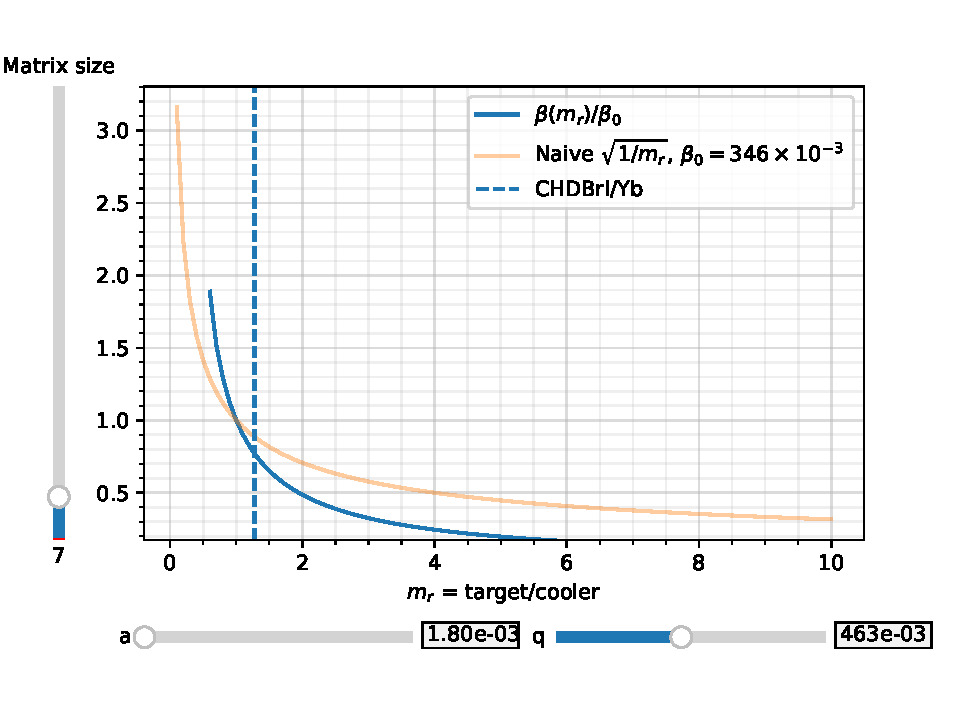
\includegraphics[width=0.95\textwidth]{graphics/software-plot-example.pdf}
	\end{center}
	\caption{An example window opened by \texttt{./plot.py}.}
	\label{fig:software-plot-example}
\end{sidewaysfigure}

\newgeometry{top=2cm, bottom=2cm}
\begin{sidewaystable}[h]
\begin{tabular}{rrrrrrrrrrrrrr}
\hline
   total $\downarrow$ &   cloud $\rightarrow$ &      0 &       1 &       2 &       3 &        4 &        5 &        6 &        7 &        8 &        9 &       10 &        11 \\
\hline
                    0 &                       &    0/1 &     0/1 &     0/1 &     0/1 &      0/1 &      0/1 &      0/1 &      0/1 &      0/1 &      0/1 &      0/1 &       1/1 \\
                    1 &                       &   0/50 &    2/50 &    3/50 &    4/50 &     5/50 &     6/50 &     8/50 &    11/50 &    14/50 &    19/50 &    25/50 &     50/50 \\
                    2 &                       &   0/72 &    3/72 &    4/72 &    6/72 &     7/72 &    10/72 &    12/72 &    16/72 &    21/72 &    27/72 &    36/72 &     72/72 \\
                    3 &                       &  0/105 &   5/105 &   6/105 &   8/105 &   11/105 &   14/105 &   18/105 &   24/105 &   31/105 &   40/105 &   52/105 &   105/105 \\
                    4 &                       &  0/153 &   7/153 &   9/153 &  12/153 &   16/153 &   21/153 &   27/153 &   35/153 &   45/153 &   59/153 &   76/153 &   153/153 \\
                    5 &                       &  0/223 &  11/223 &  14/223 &  18/223 &   24/223 &   31/223 &   40/223 &   51/223 &   66/223 &   86/223 &  111/223 &   223/223 \\
                    6 &                       &  0/325 &  16/325 &  20/325 &  27/325 &   35/325 &   45/325 &   58/325 &   75/325 &   97/325 &  125/325 &  162/325 &   325/325 \\
                    7 &                       &  0/472 &  23/472 &  30/472 &  39/472 &   50/472 &   65/472 &   84/472 &  109/472 &  141/472 &  182/472 &  236/472 &   472/472 \\
                    8 &                       &  0/687 &  34/687 &  44/687 &  57/687 &   74/687 &   95/687 &  123/687 &  159/687 &  205/687 &  265/687 &  343/687 &   687/687 \\
                    9 &                       & 0/1000 & 50/1000 & 64/1000 & 83/1000 & 107/1000 & 139/1000 & 179/1000 & 232/1000 & 299/1000 & 387/1000 & 500/1000 & 1000/1000 \\
\hline
\end{tabular}

\caption{The list of clouds' amounts. Calculated via rounding down cloud concentrations, and total amounts. Created using \texttt{./sim.py --list latex-amounts}.}
\label{tbl:sim-list-amounts}
\end{sidewaystable}
\restoregeometry
